\documentclass[11pt]{article}

\newcommand{\yourname}{}
\newcommand{\yourcollaborators}{}

\def\comments{0}

%format and packages%\usepackage{algorithm, algorithmic}
\usepackage{algpseudocode}
\usepackage{amsmath, amssymb, amsthm}
\usepackage{enumerate}
\usepackage{enumitem}
\usepackage{framed}
\usepackage{verbatim}
\usepackage[margin=1.0in]{geometry}
\usepackage{multirow}

\usepackage{microtype}


\usepackage{graphicx}
\usepackage{tikz}
\usetikzlibrary{automata, positioning, arrows.meta}

	\definecolor{processblue}{cmyk}{0.96,0,0,0}


\usepackage{kpfonts}
\usepackage{palatino}
	\DeclareMathAlphabet{\mathtt}{OT1}{cmtt}{m}{n}
	\SetMathAlphabet{\mathtt}{bold}{OT1}{cmtt}{bx}{n}
	\DeclareMathAlphabet{\mathsf}{OT1}{cmss}{m}{n}
	\SetMathAlphabet{\mathsf}{bold}{OT1}{cmss}{bx}{n}
	\renewcommand*\ttdefault{cmtt}
	\renewcommand*\sfdefault{cmss}
	\renewcommand{\baselinestretch}{1.06}
\usepackage{tikz}
	\usetikzlibrary{positioning}
	\definecolor{processblue}{cmyk}{0.96,0,0,0}
    \usetikzlibrary{matrix,arrows}

\tikzset{
->, % makes the edges directed
>=Stealth, % makes the arrow heads bold
node distance=3cm, % specifies the minimum distance between two nodes. Change if necessary.
every state/.style={thick, fill=gray!10}, % sets the properties for each ’state’ node
initial text=$ $, % sets the text that appears on the start arrow
}
	
\usepackage{hyperref}

\hypersetup{
	linktocpage=true,
	colorlinks=true,				% false: boxed links; true: colored links
	linkcolor=blue,		% color of internal links
	citecolor=blue,	% color of links to bibliography
	urlcolor=blue,		% color of external links
}

\usepackage[boxruled,vlined,nofillcomment]{algorithm2e}
	\SetKwProg{Fn}{Function}{\string:}{}
	\SetKwFor{While}{While}{}{}
	\SetKwFor{For}{For}{}{}
	\SetKwIF{If}{ElseIf}{Else}{If}{:}{ElseIf}{Else}{:}
	\SetKw{Return}{Return}

%enclosure macros
\newcommand{\paren}[1]{\ensuremath{\left( {#1} \right)}}
\newcommand{\bracket}[1]{\ensuremath{\left\{ {#1} \right\}}}
\renewcommand{\sb}[1]{\ensuremath{\left[ {#1} \right\]}}
\newcommand{\ab}[1]{\ensuremath{\left\langle {#1} \right\rangle}}

%probability macros
\newcommand{\ex}[2]{{\ifx&#1& \mathbb{E} \else \underset{#1}{\mathbb{E}} \fi \left[#2\right]}}
\newcommand{\pr}[2]{{\ifx&#1& \mathbb{P} \else \underset{#1}{\mathbb{P}} \fi \left[#2\right]}}
\newcommand{\var}[2]{{\ifx&#1& \mathrm{Var} \else \underset{#1}{\mathrm{Var}} \fi \left[#2\right]}}

%useful CS macros
\newcommand{\poly}{\mathrm{poly}}
\newcommand{\polylog}{\mathrm{polylog}}
\newcommand{\zo}{\{0,1\}}
\newcommand{\pmo}{\{\pm1\}}
\newcommand{\getsr}{\gets_{\mbox{\tiny R}}}
\newcommand{\card}[1]{\left| #1 \right|}
\newcommand{\set}[1]{\left\{#1\right\}}
\newcommand{\negl}{\mathrm{negl}}
\newcommand{\eps}{\varepsilon}
\DeclareMathOperator*{\argmin}{arg\,min}
\DeclareMathOperator*{\argmax}{arg\,max}
\newcommand{\eqand}{\qquad \textrm{and} \qquad}
\newcommand{\ind}[1]{\mathbb{I}\{#1\}}
\newcommand{\sslash}{\ensuremath{\mathbin{/\mkern-3mu/}}}

%mathbb
\newcommand{\N}{\mathbb{N}}
\newcommand{\R}{\mathbb{R}}
\newcommand{\Z}{\mathbb{Z}}
%mathcal
\newcommand{\cA}{\mathcal{A}}
\newcommand{\cB}{\mathcal{B}}
\newcommand{\cC}{\mathcal{C}}
\newcommand{\cD}{\mathcal{D}}
\newcommand{\cE}{\mathcal{E}}
\newcommand{\cF}{\mathcal{F}}
\newcommand{\cL}{\mathcal{L}}
\newcommand{\cM}{\mathcal{M}}
\newcommand{\cO}{\mathcal{O}}
\newcommand{\cP}{\mathcal{P}}
\newcommand{\cQ}{\mathcal{Q}}
\newcommand{\cR}{\mathcal{R}}
\newcommand{\cS}{\mathcal{S}}
\newcommand{\cU}{\mathcal{U}}
\newcommand{\cV}{\mathcal{V}}
\newcommand{\cW}{\mathcal{W}}
\newcommand{\cX}{\mathcal{X}}
\newcommand{\cY}{\mathcal{Y}}
\newcommand{\cZ}{\mathcal{Z}}

\newcommand{\opt}{\textsc{opt}}

%theorem macros
\newtheorem{thm}{Theorem}
\newtheorem{lem}[thm]{Lemma}
\newtheorem{fact}[thm]{Fact}
\newtheorem{clm}[thm]{Claim}
\newtheorem{rem}[thm]{Remark}
\newtheorem{coro}[thm]{Corollary}
\newtheorem{prop}[thm]{Proposition}
\newtheorem{conj}[thm]{Conjecture}

\theoremstyle{definition}
\newtheorem{defn}[thm]{Definition}


\newcommand{\instructor}{Drew van der Poel}
\newcommand{\hwnum}{1}
\newcommand{\hwdue}{Friday, July 15 at 11:59pm via \href{https://www.gradescope.com/courses/406943}{Gradescope}}

\theoremstyle{theorem}
\newtheorem{prob}{Problem}
\newtheorem{sol}{Solution}

\definecolor{cit}{rgb}{0.05,0.2,0.45} 
\newcommand{\solution}{\medskip\noindent{\color{blue}\textbf{Solution:}}}

\begin{document}
{\Large 
\begin{center}{CS3800: Theory of Computation} --- Summer II '22 --- \instructor \end{center}}
{\large
\vspace{10pt}
\noindent Homework~\hwnum \vspace{2pt}\\
Due~\hwdue}

\bigskip
{\large
\noindent Name: \yourname \vspace{2pt}\\ Collaborators: \yourcollaborators}

\vspace{15pt}
\begin{itemize}

\item Make sure to put your name on the first page.  If you are using the \LaTeX~template we provided, then you can make sure it appears by filling in the \texttt{yourname} command.

\item This assignment is due~\hwdue.  No late assignments will be accepted.  Make sure to submit something before the deadline.

\item Solutions must be typeset.  If you need to draw any diagrams, you may draw them by hand as long as they are embedded in the PDF.  I recommend using the source file for this assignment to get started.

\item I encourage you to work with your classmates on the homework problems. \emph{If you do collaborate, you must write all solutions by yourself, in your own words.}  Do not submit anything you cannot explain.  Please list all your collaborators in your solution for each problem by filling in the \texttt{yourcollaborators} command.

\item Finding solutions to homework problems on the web, or by asking students not enrolled in the class is strictly forbidden.

\end{itemize}



\newpage

\begin{prob} Automata: Element Ranges (\emph{4 points})\end{prob}


\begin{enumerate}[label=(\alph*)]

\item \textbf{[2 points]}   In a DFA with 10 states and an alphabet of size 6, what is the range on the number of transitions? What is the range on the number of start states and accept states? A transition is defined as a state-symbol pair mapped to a state $(q \in Q, c \in \Sigma) \rightarrow (r \in Q)$. Briefly justify your answer.

\solution

A DFA with 10 states and an alphabet of size 6 will have ONLY 60 transitions, every "letter" in the alphabet will have a transition with each of the 10 states in the DFA or $6 * 10$ number of transitions. Anymore or any less transitions and the DFA will be have to be considered a NFA.
\\[3ex] The number of start states per definition of a DFA has to be 1.
\\[3ex] The number of accept states is in the range of $[0, 10]$ since there can be as many all of the states being accept states and as a few as none of the states being accept states.


\item \textbf{[2 points]}    In a NFA with 10 states and an alphabet of size 6, what is the range on the number of transitions? What is the range on the number of start states and accept states? A transition is defined as a state-symbol pair mapped to a state $(q \in Q, c \in \Sigma \cup \epsilon) \rightarrow (r \in Q)$. You can assume there are no $\epsilon$-transitions from a state to itself. Briefly justify your answer.


\solution

The number of transitions in a NFA with 10 states and an alphabet size of 6 is in the range of $[0, 690]$. The lower bound is 0 because it's entirely possible for the entire NFA to have 0 transitions for each character in the alphabet.
The upper bound is 690 because for each given state, each character can have a transition from that state to every state (including itself) in the NFA so that gives $(1$ character $* 10$ possible states $)$ $*$ $(6$ characters in the alphabet$)$ = 600.
However there are also $\epsilon$-transitions and given the assumption that "there are no $\epsilon$-transitions from a state to itself" then each state can have an $\epsilon$-transition from itself to every other state which means that in total, there are ((10 - 1) $\epsilon$-transition per state) * (10 states) = 90.
Adding it all up, the upper-bound number of transitions in this NFA would be $690$.
\\[3ex] The number of starts states per definition of a NFA has to be 1.
\\[3ex] The number of accept states is in the range of $[0, 10]$ since there can be as many all of the states being accept states and as a few as none of the states being accept states.


\end{enumerate}


\newpage

\begin{prob} What Language? (\emph{4 points})\end{prob}

Determine the language that the following DFA recognizes. Briefly justify your answer.

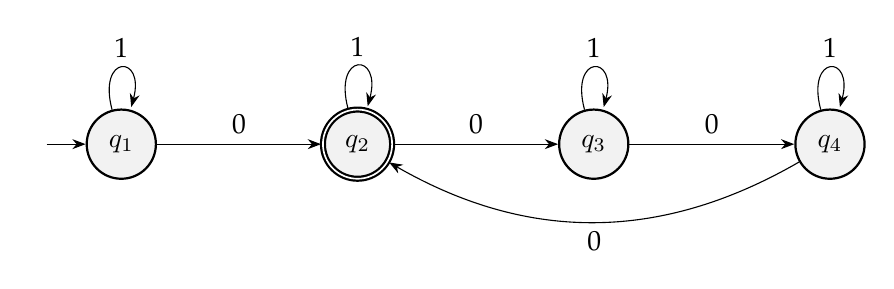
\begin{tikzpicture}
\node[state, initial] (q1) {$q_1$};
\node[state, accepting, right of=q1] (q2) {$q_2$};
\node[state, right of=q2] (q3) {$q_3$};
\node[state, right of=q3] (q4) {$q_4$};
\draw (q1) edge[loop above] node{1} (q1)
(q1) edge[above] node{0} (q2)
(q2) edge[loop above] node{1} (q2)
(q2) edge[above] node{0} (q3)
(q3) edge[loop above] node{1} (q3)
(q3) edge[above] node{0} (q4)
(q4) edge[bend left] node [below] {0} (q2)
(q4) edge[loop above] node{1} (q4);
\end{tikzpicture}

\solution
\\Example Inputs:\\
"0" $\rightarrow$ ACCEPT \\\\
"00" $\rightarrow$ REJECT \\\\
"0000" $\rightarrow$ ACCEPT \\\\
"011111111111" $\rightarrow$ ACCEPT (number of 1's doesn't matter) \\\\
"01000" $\rightarrow$ACCEPT \\\\
"00000" $\rightarrow$ REJECT \\

\noindent Defining the above DFA as $M$ then the $L(M)$ = \{ $w$ $|$ the number of zeroes in $w$ modulo 3 is 1 \} 


\newpage

\begin{prob} Draw a DFA (\emph{6 points})\end{prob}


Consider the following language $L$ over $\Sigma = \{0, 1\}$. \\

$L = \{x | $ any two 0s in $x$ are separated by at least three 1s $\}$\\

For example, $01110, 01111011101111101, 11101, 1111$ are all in $L$, but $00, 0110, 01110110$ are not.\\

Draw a DFA which recognizes $L$. Be sure to include all states and transitions and to denote the start and accept states. Your DFA should accept the empty string. Your DFA should be as simple as possible.

\solution






\newpage

\begin{prob} Union (\emph{10 points})\end{prob}

Let $\Sigma = \{a,b\}$. Let $L1$ be the language consisting of strings where all a's are before all b's. Let $L2$ be the language consisting of strings where the number of a's is odd. Draw DFAs recognizing each language, then use the construction seen in class to draw a DFA recognizing $L1 \cup L2$.



\solution

\noindent Let $M_1$ be the DFA that recognizes $L1$ \\
\noindent Let $M_2$ be the DFA that recognizes $L2$ \\
\noindent Let $M_3$ be the DFA that recognizes $L1 \cup L2$ where state, $(e, r)$, is a state-pair where $e$ is from $M_1$ and $r$ is from $M_2$ 
 



\newpage

\begin{prob} NFAs (\emph{6 points})\end{prob}


 Consider the alphabet $\Sigma = \{o, t, w\}$. Let $L$ be the language of strings which are concatenations of ``to", ``too", and ``two".  Draw a NFA which recognizes $L$. Your NFA should make use of $\epsilon$-transitions and/or have state-character pairs with 0 or more than 1 transitions (to truly take advantage of using NFAs!).  Your NFA should accept the empty string.

\solution




\end{document}
